
The given system of inequality can be written in matrix form as
\begin{align}
    \myvec{-1 & -2  \\ -1 & 1 \\ 1 & 1\\ 1 & 0 \\ 0 & 1}\vec{x} \succeq \myvec{-10\\0\\1\\0\\0}
\end{align}
which can be further simplified into 
\begin{align}
    \myvec{-1 & -2 \\ 1 & 0 \\ 0&1}\vec{x} \succeq \myvec{-10\\\frac{-1}{2}\\\frac{-1}{2}}
\end{align}
Let the surplus vector be
\begin{align}
    \vec{u} &= \myvec{u_1\\u_2} \succeq 0
\end{align}
\begin{enumerate}
    \item 
    \begin{align}
        \myvec{-1 & -2 \\ 1 & 0}\vec{x} &\succeq \myvec{-10 \\ \frac{-1}{2}}
        \\
        \implies  \myvec{-1 & -2 \\ 1 & 0}\vec{x} &= \myvec{-10 \\ \frac{-1}{2}} + \vec{u}
    \end{align}
    resulting in 
    \begin{align}
        \vec{x} &= \myvec{-1 & -2 \\ 1 & 0}^{-1}\myvec{-10 \\\frac{-1}{2}} + \myvec{-1 & -2 \\ 1 & 0}^{-1}\vec{u}
        \\
        \implies \vec{x} &= \myvec{\frac{1}{2} \\ \frac{19}{4}} + \myvec{0&1\\ \frac{-1}{2}&\frac{-1}{2}}\vec{u}   \label{ineq/58/eq1}
    \end{align}
    \item 
    \begin{align}
        \myvec{-1& -2 \\ 0 & 1}\vec{x} &\succeq \myvec{-10 \\ \frac{-1}{2}}
        \\
        \implies  \myvec{-1& -2 \\ 0 & 1}\vec{x} &= \myvec{-10 \\ \frac{-1}{2}} + \vec{u}
    \end{align}
    resulting in 
    \begin{align}
        \vec{x} &= \myvec{-1& -2 \\ 0 & 1}^{-1}\myvec{-10 \\ \frac{-1}{2}} + \myvec{-1& -2 \\ 0 & 1}^{-1}\vec{u}
        \\
        \implies \vec{x} &= \myvec{9\\\frac{1}{2}} + \myvec{-1& -2 \\ 0 & 1}\vec{u} \label{ineq/58/eq2}
    \end{align}
\end{enumerate}
Now,solution region which is common to regions of eq. \eqref{ineq/58/eq1} and eq. \eqref{ineq/58/eq2},is given by
\begin{align}
    \boxed{\vec{x} = \myvec{\frac{1}{2}\\\frac{1}{2}}+\myvec{0&1\\\frac{-1}{2}&1}\vec{u}}
\end{align}
%
\begin{figure}[!ht]
\centering
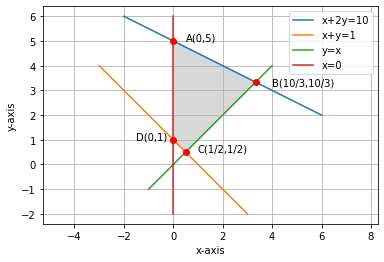
\includegraphics[width=\columnwidth]{solutions/su2021/2/58/Figures/Figure_2.58.png}
\caption{Graphical Solution}
\label{ineq/58/fig:fig1}	
\end{figure}

\begin{figure}[!ht]
\centering
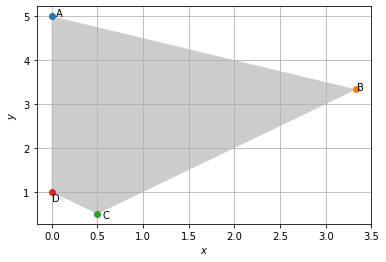
\includegraphics[width=\columnwidth]{solutions/su2021/2/58/Figures/2.58(2).png}
\caption{Magnified Solution region}
\label{ineq/58/fig:fig2}	
\end{figure}

